\documentclass[10pt]{article}
\usepackage[margin=0.75in]{geometry}
\usepackage{graphicx,booktabs,amsmath,float}
\usepackage[font=small]{caption}
\begin{document}
\begin{center}{\Large\bf Feature importance of the 15:30 forecast (16:00 bar)}\\[3pt]
{\small MDI, split count, permutation importance on the causal held-out tail, SHAP --- trees and the per-bar linear models; 1,469 forecasts 2018-06-25 .. 2024-04-30, 147 refits}\end{center}

\textbf{Setup.} Models: per-bar ridge and lasso (coefficients re-solved every session, penalty re-chosen causally every 250 sessions) and the untuned per-bar LightGBM, XGBoost and random forest (refit every 10 sessions) --- the shipped configurations. Every fit uses the 2000 sessions before it. A refit's \emph{held-out tail} is the $\le 10$ sessions its model forecasts, up to the next refit: never in its fit, so a loss change measured there is out of sample and causal. Buckets: all features, and HAR + calendar. Library: scikit-learn 1.9.0 (random forest), LightGBM 4.6.0, XGBoost 3.2.0, shap 0.51.0; the permutation and drop-column loops are written out, because a library permutation routine scores one fitted model on one test set, not 147 walk-forward models on their own tails.

\textbf{Measures.} (1) \emph{MDI / gain}: LightGBM gain, XGBoost total gain, random-forest impurity decrease; share per refit, averaged. (2) \emph{Split count}. (3) \emph{Permutation importance} on the tail, loss = QLIKE of the plain back-transform $\hat y^2\times$ diurnal baseline against the bar's realized variance (no recalibration), and squared error in the fit space; 10 draws per unit and refit, the same draws for all five models. P1 shuffles the unit's values among the tail's rows (the literal permutation; blind to slow inputs, which barely move in 10 sessions); P2 replaces them with rows drawn from the refit's own training window (past data only). A unit is a column, a \emph{series} (all columns of one input: lags, flags, gates) or a \emph{cluster} (columns every pair of which has $|$corr$|\ge 0.8$, complete linkage); a group's columns move together. Intervals: 95\% circular-block bootstrap over refits (block 6). (4) \emph{SHAP}: TreeSHAP (path-dependent) on the same tail rows; for the linear models $\beta_j(x_j-\bar x_j)$ with the window mean as background. Linear extras: $|\beta\cdot sd|$ and drop-column importance (re-solve without the unit, penalty held).

\textbf{Key.} \texttt{har\_ma\_*} realized variance of the bar (the target's own HAR ladder, means over the last 1, 5, 25, 125, 625, 3125 bars; \texttt{har\_ma\_*\_x\_close} = the same times the 16:00 close gate, identical at this bar); \texttt{adj\_sumabsret\_ma\_*} absolute return; \texttt{adj\_sumret\_ma\_*} signed return; \texttt{adj\_sumret3/4\_ma\_*} 3rd/4th-power returns; \texttt{adj\_sumpret2\_ma\_*} upside squared returns; \texttt{adj\_sumbipow\_ma\_*} bipower variation; \texttt{adj\_sumautocov\_ma\_*} return autocovariance; \texttt{adj\_sumvolume\_ma\_*} ES volume; \texttt{adj\_numobs\_ma\_*} ES prints per bar; \texttt{adj\_vix/vvix/vix3m\_ma\_*} the Cboe indices; \texttt{adj\_fomc\_*} FOMC flags and distances; \texttt{*\_avail/active\_ma\_*} is-present / is-nonzero flags; calendar = \texttt{DOW\_*}, \texttt{is\_*}, \texttt{hour}, \texttt{days\_to\_opex}. all features adds the constituent cross-section (\texttt{*\_ewstock}, \texttt{*\_vwstock}), Cboe volume (\texttt{adj\_voldemand\_*}) and StockTwits (\texttt{adj\_stocktwits\_*}).

\begin{table}[H]\centering\footnotesize
\caption{The design is float throughout, but not all continuous: distinct values per column in each 2000-session window (median over the 147 windows) --- what MDI's cardinality bias keys on.}
\begin{tabular}{lrrrrrrrr}\toprule
bucket & columns & constant & binary & 3--25 & 26--500 & $>$500 & series & clusters (columns)\\\midrule
HAR + calendar & 34 & 10 & 11 & 0 & 1 & 12 & 2 & 5 (14) \\
all features & 640 & 143 & 40 & 93 & 91 & 273 & 49 & 101 (505) \\
\bottomrule\end{tabular}\end{table}

\section*{1. Does MDI's cardinality bias matter here? Yes, below the leader.}
\begin{table}[H]\centering\footnotesize
\caption{Spearman rank correlation, over the non-constant columns, between a column's importance and its number of distinct values. MDI, split count and TreeSHAP track cardinality; permutation importance does not.}
\begin{tabular}{llrrrrrr}\toprule
bucket & model & MDI & split & SHAP & perm P1 QL & perm P2 QL & perm P2 MSE\\\midrule
all features & LightGBM & 0.84 & 0.84 & 0.81 & 0.02 & -0.06 & -0.03 \\
all features & XGBoost & 0.83 & 0.83 & 0.81 & 0.19 & 0.17 & 0.06 \\
all features & random forest & 0.90 & 0.91 & 0.88 & 0.08 & 0.05 & -0.02 \\
HAR + calendar & LightGBM & 0.85 & 0.84 & 0.72 & 0.23 & 0.20 & 0.04 \\
HAR + calendar & XGBoost & 0.79 & 0.79 & 0.73 & 0.33 & 0.43 & 0.41 \\
HAR + calendar & random forest & 0.86 & 0.83 & 0.80 & 0.11 & 0.38 & 0.57 \\
\bottomrule\end{tabular}\end{table}
\begin{table}[H]\centering\scriptsize
\caption{Noise probes: on every third refit a second fit appends three pure-noise columns (continuous; 20 values; binary). Median rank among all columns (1 = most important) and, in brackets, the share of the real columns the model uses that rank below the probe; permutation P2 of the continuous probe ($\Delta$QLIKE $\times 10^{3}$, 95\% interval) against \texttt{har\_ma\_*}'s.}
\begin{tabular}{llrrrrrrrr}\toprule
bucket & model & cols & MDI rank & split rank & SHAP rank & 20-val MDI & binary MDI & perm P2 (cont.) & \texttt{har\_ma\_*}\\\midrule
all features & LightGBM & 643 & 77 (75\%) & 47 (83\%) & 100 (69\%) & 153 & 319 & $-0.08$ [-0.33, +0.14] & 294 \\
all features & XGBoost & 643 & 117 (64\%) & 80 (72\%) & 131 (60\%) & 166 & 319 & $+0.17$ [+0.01, +0.38] & 280 \\
all features & random forest & 643 & 48 (89\%) & 10 (98\%) & 92 (79\%) & 108 & 317 & $-0.04$ [-0.40, +0.33] & 368 \\
HAR + calendar & LightGBM & 37 & 8 (72\%) & 5 (84\%) & 11 (60\%) & 11 & 16 & $+0.08$ [-1.51, +1.81] & 630 \\
HAR + calendar & XGBoost & 37 & 9 (64\%) & 6 (80\%) & 13 (51\%) & 13 & 19 & $+0.50$ [-0.22, +1.17] & 588 \\
HAR + calendar & random forest & 37 & 5 (80\%) & 1 (100\%) & 11 (60\%) & 9 & 15 & $-0.35$ [-2.26, +1.60] & 691 \\
\bottomrule\end{tabular}\end{table}

\textbf{Reading.} A column of pure noise with a new value on every row is ranked by MDI above 75\%, 64\%, 89\% (LightGBM, XGBoost, forest) of the real all-features columns the model uses, and by the forest's split count above 98\%; the binary noise column sits near the bottom. The same noise gets a permutation importance of at most 0.50$\times10^{-3}$ in absolute value (5 of 6 intervals include zero; the exceptions all features XGBoost [+0.01, +0.38]e-3), against at least 0.28 for \texttt{har\_ma\_*}. TreeSHAP, which splits the fitted trees, inherits part of the bias. Over the real columns, MDI, split count and SHAP correlate 0.83--0.88 with the number of distinct values, permutation -0.06--0.19. So below the leader, the MDI / split ranking of this design is partly a ranking by cardinality; the permutation ranking is the one to use for selection. At the series level the bias does not reach the top: every tree measure puts \texttt{har\_ma\_*} first. Series that MDI or split count puts in the top 5 but permutation P2 ranks outside the top 10 (permutation rank in brackets): all features LightGBM: \texttt{adj\_sellturnover\_vwstock\_ma\_*} (35), \texttt{adj\_stocktwits\_sentiment\_ma\_*} (49), \texttt{adj\_sumret3\_ma\_*} (28); all features XGBoost: \texttt{adj\_sumautocov\_ma\_*} (11); all features random forest: \texttt{adj\_voldemand\_spx\_open\_and\_close\_ma\_*} (47), \texttt{adj\_voldemand\_all\_open\_only\_ma\_*} (36), \texttt{adj\_voldemand\_spx\_open\_only\_ma\_*} (43).

\section*{2. The top inputs by measure}
\begin{table}[H]\centering\scriptsize
\caption{All-features design, series level: top three per model and measure (share for MDI / split / $|\beta\cdot sd|$ / SHAP; change as \% of the model's tail loss for permutation and drop-column).}
\begin{tabular}{llp{11.2cm}}\toprule
model & measure & top three\\\midrule
ridge & $|\beta\cdot sd|$ & \texttt{har\_ma\_*} 11\%; \texttt{adj\_sumabsret\_ma\_*} 5\%; \texttt{adj\_sumabsret\_vwstock\_ma\_*} 5\% \\
ridge & perm.\ P1, $\Delta$MSE & \texttt{har\_ma\_*} +63\%; \texttt{adj\_sumabsret\_ma\_*} +7\%; \texttt{adj\_sumabsret\_vwstock\_ma\_*} +7\% \\
ridge & perm.\ P2, $\Delta$MSE & \texttt{har\_ma\_*} +142\%; \texttt{adj\_sumabsret\_ma\_*} +22\%; \texttt{adj\_sumabsret\_vwstock\_ma\_*} +18\% \\
ridge & perm.\ P2, $\Delta$QLIKE & \texttt{adj\_sumautocov\_ma\_*} +4051120\%; \texttt{adj\_spread\_vwstock\_ma\_*} +57340\%; \texttt{adj\_voldemand\_spx\_open\_only\_ma\_*} +3749\% \\
ridge & drop-column, $\Delta$MSE & \texttt{har\_ma\_*} +17\%; \texttt{calendar} +2\%; \texttt{adj\_sumvolume\_ma\_*} +2\% \\
ridge & SHAP mean $|\phi|$ & \texttt{har\_ma\_*} 15\%; \texttt{adj\_sumabsret\_ma\_*} 6\%; \texttt{adj\_sumabsret\_vwstock\_ma\_*} 5\% \\
lasso & $|\beta\cdot sd|$ & \texttt{har\_ma\_*} 46\%; \texttt{adj\_sumabsret\_vwstock\_ma\_*} 10\%; \texttt{adj\_sumret\_ma\_*} 9\% \\
lasso & perm.\ P1, $\Delta$MSE & \texttt{har\_ma\_*} +145\%; \texttt{adj\_sumabsret\_vwstock\_ma\_*} +8\%; \texttt{adj\_sumret\_ma\_*} +7\% \\
lasso & perm.\ P2, $\Delta$MSE & \texttt{har\_ma\_*} +290\%; \texttt{adj\_sumabsret\_vwstock\_ma\_*} +18\%; \texttt{adj\_vix\_ma\_*} +15\% \\
lasso & perm.\ P2, $\Delta$QLIKE & \texttt{har\_ma\_*} +259\%; \texttt{adj\_vix3m\_ma\_*} +85\%; \texttt{adj\_sumbipow\_ewstock\_ma\_*} +48\% \\
lasso & drop-column, $\Delta$MSE & \texttt{har\_ma\_*} +27\%; \texttt{adj\_sumret\_ma\_*} +2\%; \texttt{adj\_sumabsret\_vwstock\_ma\_*} +1\% \\
lasso & SHAP mean $|\phi|$ & \texttt{har\_ma\_*} 46\%; \texttt{adj\_sumabsret\_vwstock\_ma\_*} 10\%; \texttt{adj\_sumret\_ma\_*} 9\% \\
LightGBM & MDI / gain & \texttt{har\_ma\_*} 57\%; \texttt{adj\_sumret\_ma\_*} 5\%; \texttt{adj\_sumabsret\_ma\_*} 4\% \\
LightGBM & split count & \texttt{har\_ma\_*} 12\%; \texttt{adj\_sumret\_ma\_*} 6\%; \texttt{adj\_sumvolume\_ma\_*} 4\% \\
LightGBM & perm.\ P1, $\Delta$QLIKE & \texttt{har\_ma\_*} +111\%; \texttt{calendar} +5\%; \texttt{adj\_sumret\_ma\_*} +4\% \\
LightGBM & perm.\ P2, $\Delta$QLIKE & \texttt{har\_ma\_*} +237\%; \texttt{calendar} +6\%; \texttt{adj\_sumret\_ma\_*} +4\% \\
LightGBM & perm.\ P2, $\Delta$MSE & \texttt{har\_ma\_*} +235\%; \texttt{calendar} +4\%; \texttt{adj\_sumret\_ma\_*} +3\% \\
LightGBM & SHAP mean $|\phi|$ & \texttt{har\_ma\_*} 47\%; \texttt{adj\_sumret\_ma\_*} 6\%; \texttt{adj\_sumvolume\_ma\_*} 4\% \\
XGBoost & MDI / gain & \texttt{har\_ma\_*} 69\%; \texttt{adj\_sumret\_ma\_*} 4\%; \texttt{adj\_sumabsret\_ma\_*} 4\% \\
XGBoost & split count & \texttt{har\_ma\_*} 21\%; \texttt{adj\_sumret\_ma\_*} 8\%; \texttt{adj\_sumvolume\_ma\_*} 5\% \\
XGBoost & perm.\ P1, $\Delta$QLIKE & \texttt{har\_ma\_*} +107\%; \texttt{adj\_sumret\_ma\_*} +4\%; \texttt{calendar} +4\% \\
XGBoost & perm.\ P2, $\Delta$QLIKE & \texttt{har\_ma\_*} +224\%; \texttt{adj\_sumret\_ma\_*} +4\%; \texttt{calendar} +4\% \\
XGBoost & perm.\ P2, $\Delta$MSE & \texttt{har\_ma\_*} +231\%; \texttt{adj\_sumret\_ma\_*} +4\%; \texttt{adj\_sumvolume\_ma\_*} +3\% \\
XGBoost & SHAP mean $|\phi|$ & \texttt{har\_ma\_*} 55\%; \texttt{adj\_sumret\_ma\_*} 7\%; \texttt{adj\_sumvolume\_ma\_*} 5\% \\
random forest & MDI / gain & \texttt{har\_ma\_*} 62\%; \texttt{adj\_sumabsret\_ma\_*} 5\%; \texttt{adj\_sumret\_ma\_*} 3\% \\
random forest & split count & \texttt{har\_ma\_*} 4\%; \texttt{adj\_voldemand\_all\_open\_and\_close\_ma\_*} 3\%; \texttt{adj\_voldemand\_spx\_open\_and\_close\_ma\_*} 3\% \\
random forest & perm.\ P1, $\Delta$QLIKE & \texttt{har\_ma\_*} +128\%; \texttt{calendar} +2\%; \texttt{adj\_sumret\_ma\_*} +2\% \\
random forest & perm.\ P2, $\Delta$QLIKE & \texttt{har\_ma\_*} +290\%; \texttt{calendar} +3\%; \texttt{adj\_sumabsret\_ma\_*} +3\% \\
random forest & perm.\ P2, $\Delta$MSE & \texttt{har\_ma\_*} +252\%; \texttt{calendar} +1\%; \texttt{adj\_sumvolume\_ma\_*} +1\% \\
random forest & SHAP mean $|\phi|$ & \texttt{har\_ma\_*} 58\%; \texttt{adj\_sumabsret\_ma\_*} 5\%; \texttt{adj\_sumret\_ma\_*} 4\% \\
\bottomrule\end{tabular}\end{table}
\begin{figure}[H]\centering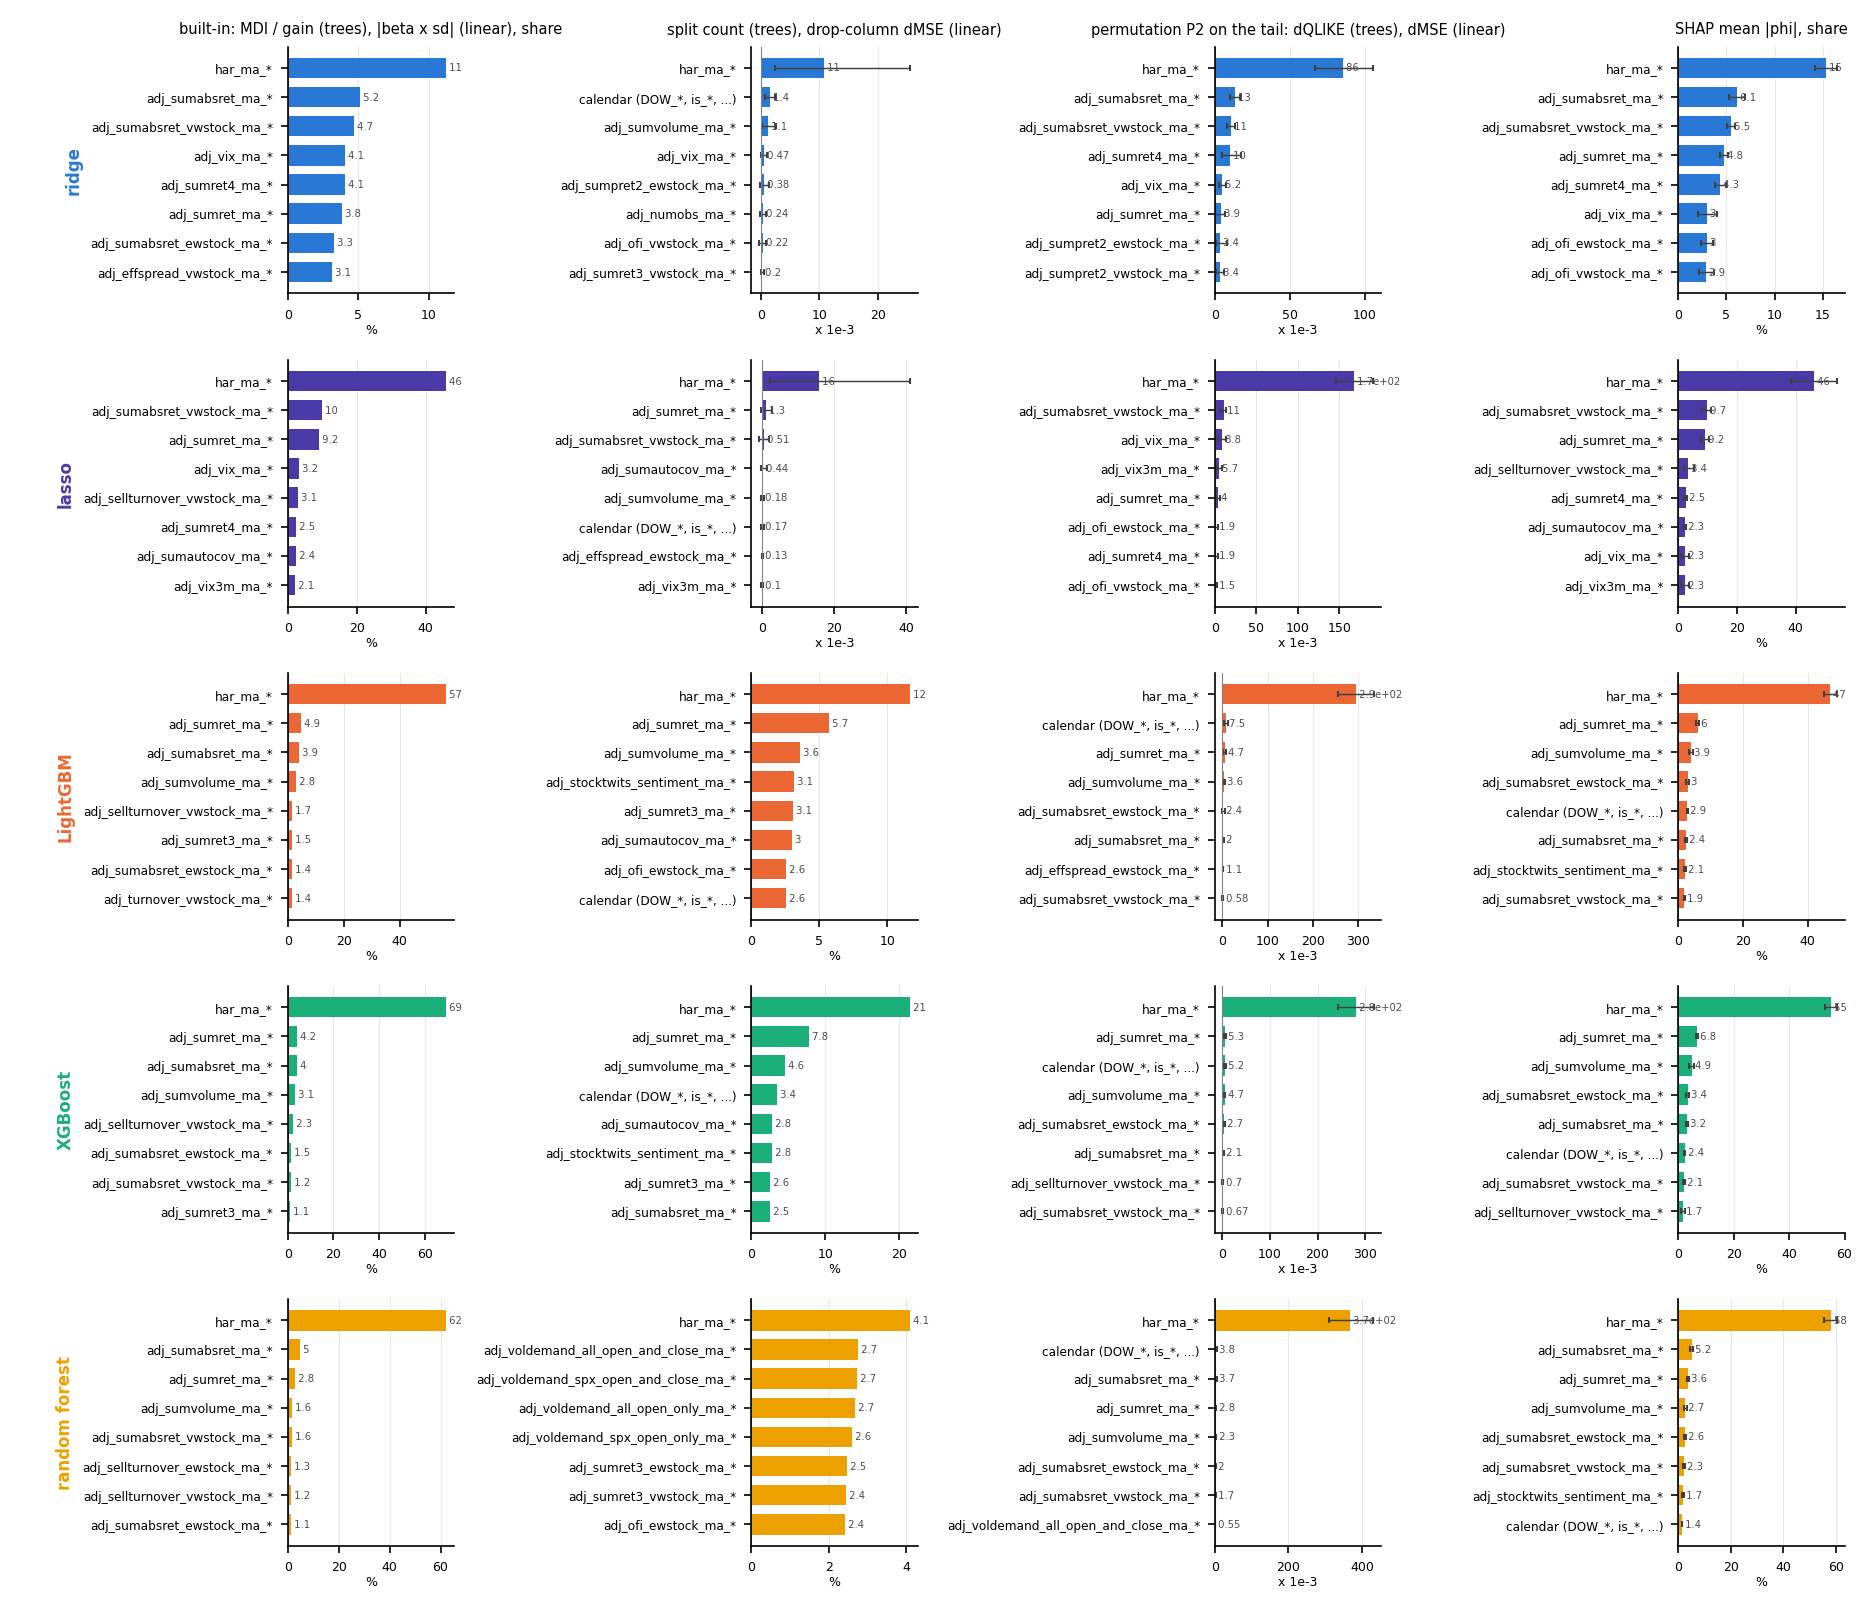
\includegraphics[width=\textwidth]{../results/feature_importance_1530/fig_ranked_all_features.png}
\caption{All features: ranked bars per measure (series level; top 8). Rows: models; columns: the built-in measure, split count (trees) / drop-column (linear), permutation P2 on the tail, SHAP. Bars with 95\% intervals over refits. Linear permutation / drop-column in $\Delta$MSE (see Section 6).}\end{figure}

\section*{3. Ranking agreement}
\begin{table}[H]\centering\scriptsize
\caption{Within a tree model: Spearman between measures (series / column level).}
\begin{tabular}{lllrrrrrr}\toprule
bucket & level & model & MDI$\sim$split & MDI$\sim$SHAP & MDI$\sim$P2 & SHAP$\sim$P2 & P1$\sim$P2 & P2 QL$\sim$MSE\\\midrule
all features & series & LightGBM & 0.87 & 0.87 & 0.22 & 0.25 & 0.75 & 0.70 \\
all features & series & XGBoost & 0.87 & 0.85 & 0.54 & 0.57 & 0.80 & 0.57 \\
all features & series & random forest & 0.64 & 0.86 & 0.22 & 0.30 & 0.67 & 0.57 \\
all features & column & LightGBM & 0.99 & 0.97 & 0.06 & 0.03 & 0.51 & 0.56 \\
all features & column & XGBoost & 0.99 & 0.97 & 0.29 & 0.28 & 0.60 & 0.45 \\
all features & column & random forest & 0.97 & 0.98 & 0.12 & 0.13 & 0.58 & 0.56 \\
\bottomrule\end{tabular}\end{table}
\begin{table}[H]\centering\scriptsize
\caption{Within a linear model: Spearman between measures.}
\begin{tabular}{lllrrrrrr}\toprule
bucket & level & model & $|\beta sd|\sim$SHAP & $|\beta sd|\sim$P2 & SHAP$\sim$P2 & P1$\sim$P2 & P2$\sim$drop & P2 QL$\sim$MSE\\\midrule
all features & series & ridge & 0.83 & 0.60 & 0.74 & 0.76 & 0.36 & 0.06 \\
all features & series & lasso & 0.95 & 0.88 & 0.86 & 0.83 & 0.16 & 0.96 \\
all features & column & ridge & 0.99 & 0.40 & 0.39 & 0.59 & 0.22 & 0.04 \\
all features & column & lasso & 0.99 & 0.32 & 0.31 & 0.61 & 0.10 & 0.78 \\
\bottomrule\end{tabular}\end{table}
\begin{table}[H]\centering\scriptsize
\caption{Across models, same measure: range of Spearman over tree--tree pairs, tree--linear pairs, and ridge--lasso.}
\begin{tabular}{llrrrrrrrrr}\toprule
bucket & level & \multicolumn{3}{c}{SHAP} & \multicolumn{3}{c}{perm P2 $\Delta$QLIKE} & \multicolumn{3}{c}{perm P2 $\Delta$MSE}\\ & & tree & tree--lin & r--l & tree & tree--lin & r--l & tree & tree--lin & r--l\\\midrule
all features & series & 0.83--0.89 & 0.33--0.49 & 0.86 & 0.43--0.59 & -0.22--0.39 & -0.04 & 0.30--0.62 & 0.04--0.45 & 0.72 \\
all features & column & 0.92--0.97 & 0.65--0.83 & 0.78 & 0.19--0.36 & -0.18--0.10 & -0.00 & 0.22--0.32 & 0.01--0.12 & 0.41 \\
\bottomrule\end{tabular}\end{table}
\begin{figure}[H]\centering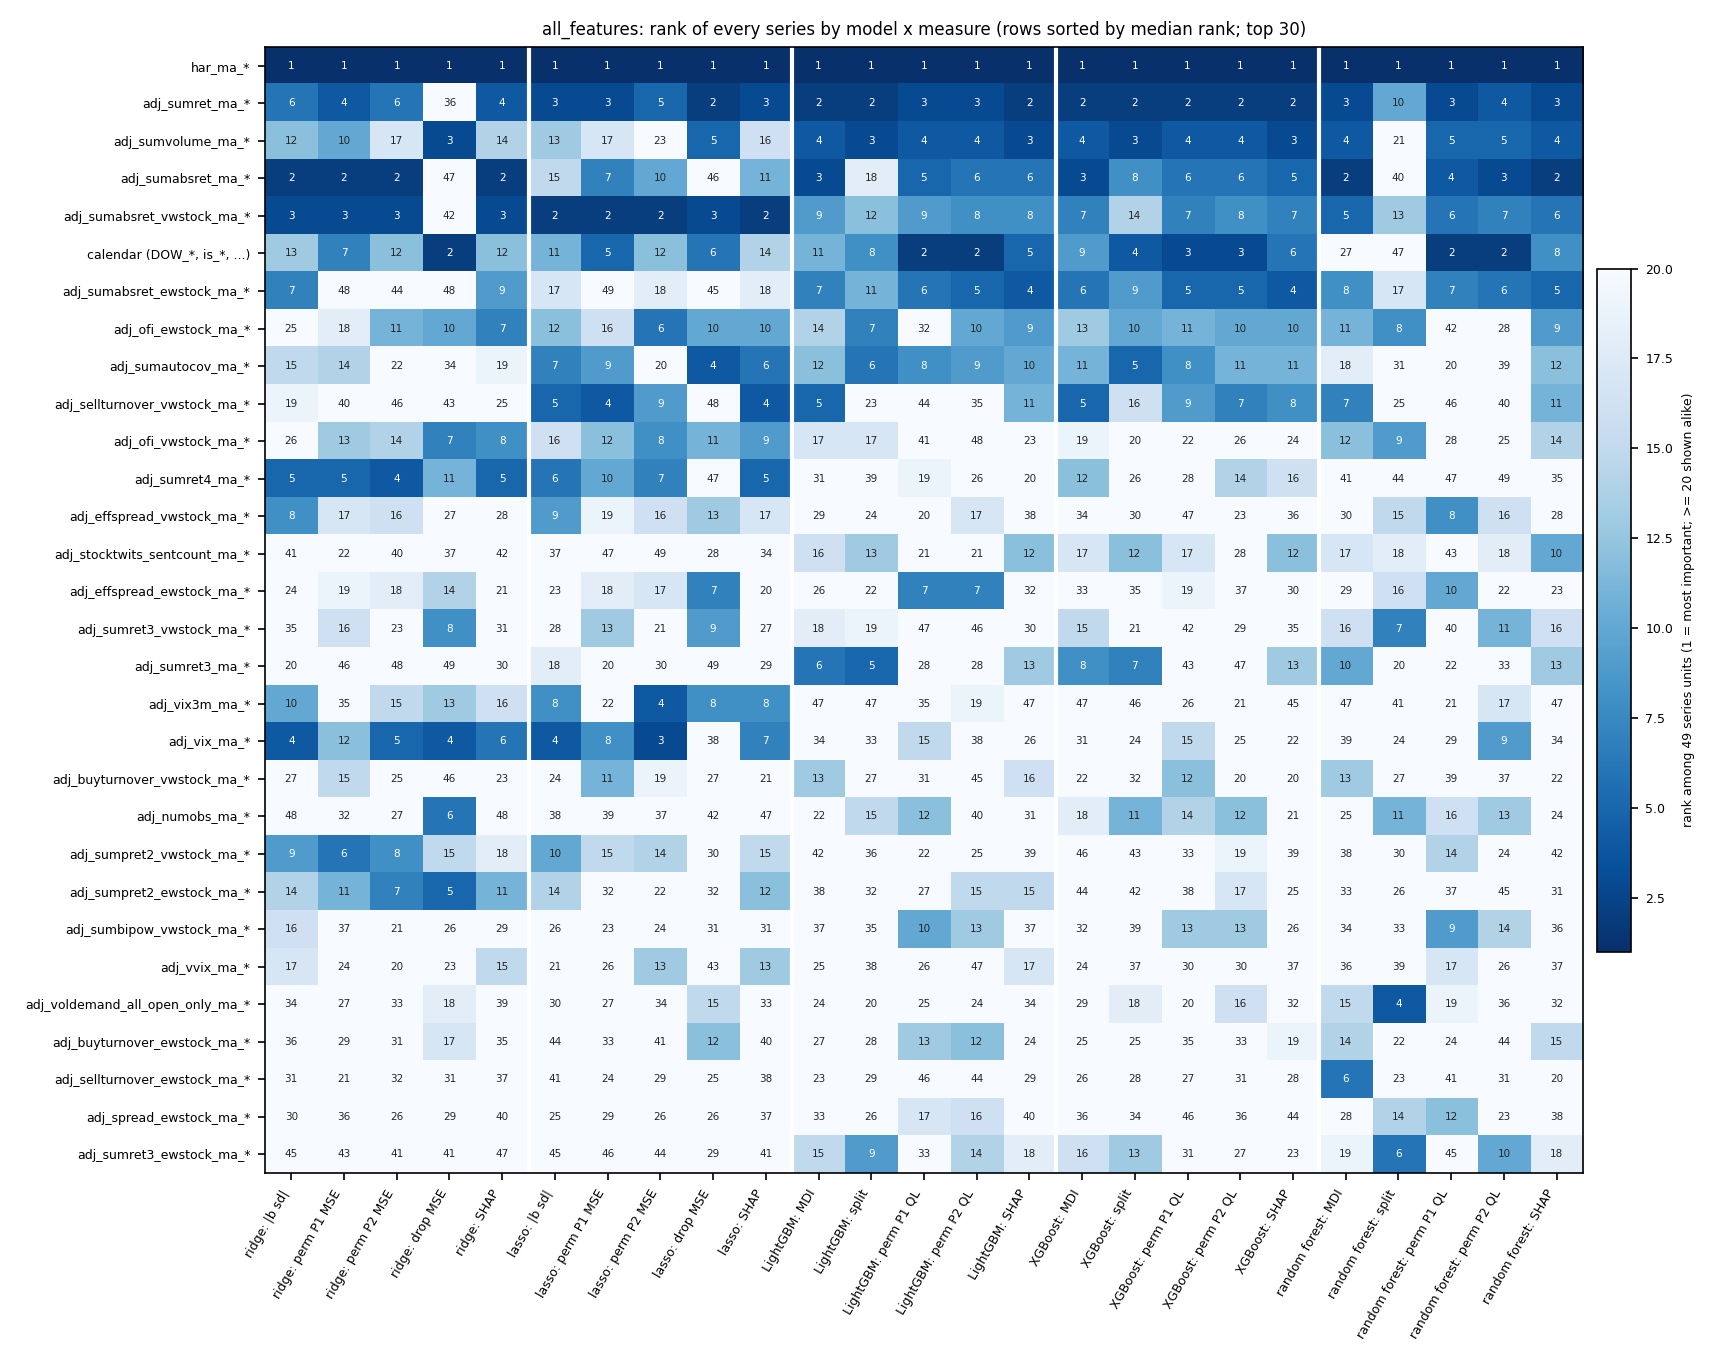
\includegraphics[width=0.95\textwidth]{../results/feature_importance_1530/fig_rank_heatmap_all_features_series.png}
\caption{All features: rank of every series under every model $\times$ measure (1 = most important).}\end{figure}

\section*{4. Stability over refits and regimes}
\begin{table}[H]\centering\scriptsize
\caption{Top-5 stability (series level): share of the 147 refits in which \texttt{har\_ma\_*} is in the refit's top 5; number of series in the top 5 in at least half the refits; number ever in the top 5. Measures: built-in (MDI or $|\beta sd|$), permutation P2 ($\Delta$QLIKE trees, $\Delta$MSE linear), SHAP.}
\begin{tabular}{llrrrrrrrrr}\toprule
bucket & model & \multicolumn{3}{c}{built-in} & \multicolumn{3}{c}{perm P2} & \multicolumn{3}{c}{SHAP}\\ & & har & $\ge$50\% & ever & har & $\ge$50\% & ever & har & $\ge$50\% & ever\\\midrule
all features & ridge & 100\% & 5 & 11 & 95\% & 3 & 40 & 99\% & 3 & 27 \\
all features & lasso & 100\% & 4 & 12 & 100\% & 3 & 31 & 100\% & 3 & 24 \\
all features & LightGBM & 100\% & 4 & 11 & 98\% & 2 & 48 & 100\% & 3 & 34 \\
all features & XGBoost & 100\% & 5 & 10 & 99\% & 3 & 45 & 100\% & 4 & 18 \\
all features & random forest & 100\% & 4 & 13 & 99\% & 1 & 47 & 100\% & 5 & 25 \\
\bottomrule\end{tabular}\end{table}
\begin{table}[H]\centering\scriptsize
\caption{Regimes: Spearman between the ranking within a stratum and the full-sample ranking (series level): median (minimum) over the calendar years (2018: 13, 2019: 26, 2020: 25, 2021: 25, 2022: 25, 2023: 25, 2024: 8 refits) and over the causal VIX terciles (VIX at 15:30 against the 1/3, 2/3 quantiles of the previous 2000 sessions' 15:30 VIX: low 28, mid 38, high 81 refits); years in which the full-sample leader also leads.}
\begin{tabular}{llrrrrrrrrr}\toprule
bucket & model & \multicolumn{3}{c}{built-in} & \multicolumn{3}{c}{perm P2} & \multicolumn{3}{c}{SHAP}\\ & & year & VIX & lead & year & VIX & lead & year & VIX & lead\\\midrule
all features & ridge & 0.93 (0.84) & 0.99 (0.95) & 7/7 & 0.69 (0.49) & 0.82 (0.58) & 7/7 & 0.76 (0.54) & 0.92 (0.83) & 7/7 \\
all features & lasso & 0.61 (0.47) & 0.99 (0.85) & 7/7 & 0.41 (0.14) & 0.75 (0.34) & 7/7 & 0.64 (0.43) & 0.97 (0.83) & 7/7 \\
all features & LightGBM & 0.95 (0.86) & 1.00 (0.99) & 7/7 & 0.56 (0.22) & 0.70 (0.67) & 7/7 & 0.83 (0.72) & 0.93 (0.92) & 7/7 \\
all features & XGBoost & 0.93 (0.88) & 0.99 (0.97) & 7/7 & 0.61 (0.10) & 0.59 (0.55) & 7/7 & 0.83 (0.67) & 0.91 (0.91) & 7/7 \\
all features & random forest & 0.98 (0.95) & 1.00 (0.99) & 7/7 & 0.55 (0.36) & 0.64 (0.42) & 7/7 & 0.90 (0.78) & 0.97 (0.96) & 7/7 \\
\bottomrule\end{tabular}\end{table}

\section*{5. Correlated inputs: the dilution caveat}
\begin{table}[H]\centering\scriptsize
\caption{Joint permutation of a cluster against the sum of its columns permuted one at a time (P2, $\Delta$MSE in the fit space $\times10^{3}$, joint / sum; squared error so the linear columns are not dominated by single tails), for the four clusters with the largest joint effect in LightGBM. Joint $>$ sum: the columns substitute for one another and one-at-a-time permutation understates the group (dilution). Joint $<$ sum: offsetting weights (permuting one column breaks an offset its partner carries).}
\begin{tabular}{llp{5.2cm}rrrrr}\toprule
bucket & cluster & members & ridge & lasso & LightGBM & XGBoost & forest\\\midrule
all features & C49 & \texttt{har\_ma\_1, har\_ma\_5, har\_ma\_1\_x\_close, har\_ma\_5\_x\_close} (4; $|r|\ge$0.89) & 33.2 / 17.6 & 85.5 / 48.9 & 101.3 / 32.0 & 96.0 / 35.4 & 136.1 / 29.0 \\
all features & C46 & \texttt{har\_ma\_25, har\_ma\_125, har\_ma\_25\_x\_close, har\_ma\_125\_x\_close} (4; $|r|\ge$0.83) & 13.4 / 7.3 & 19.9 / 11.8 & 6.3 / 2.9 & 7.0 / 3.5 & 3.0 / 1.5 \\
all features & C50 & \texttt{adj\_sumabsret\_ewstock\_ma\_1, adj\_sumabsret\_ewstock\_ma\_5, adj\_sumabsret\_vwstock\_ma\_1, adj\_sumabsret\_vwstock\_ma\_5} (4; $|r|\ge$0.85) & 15.7 / 3.0 & 8.8 / 6.5 & 1.2 / 0.2 & 0.8 / -0.3 & 1.4 / 0.1 \\
all features & C48 & \texttt{adj\_sumvolume\_ma\_1, adj\_sumvolume\_ma\_5} (2; $|r|\ge$0.89) & 1.1 / 1.4 & 0.5 / 0.6 & 0.8 / 0.5 & 1.3 / 1.0 & 0.5 / 0.5 \\
\bottomrule\end{tabular}\end{table}

\section*{6. Linear models: QLIKE permutation is dominated by single tails}
The linear forecasts are unbounded: moving an extreme input (a crash day's 4th-power or absolute return) onto another row can push the fit-space forecast through zero, and QLIKE of $\hat y^2\times$ baseline explodes. Every permutation / drop-column table therefore carries the median refit and the largest single-refit share of the sum, and the linear figures and cross-model comparisons use the squared-error versions. Trees cannot extrapolate beyond the training range of the target, so their QLIKE changes are well behaved.
\begin{table}[H]\centering\scriptsize
\caption{The top linear QLIKE entries: mean [95\% interval], median refit, share of the sum carried by one refit.}
\begin{tabular}{lllllrr}\toprule
bucket & model & measure & top series & mean [interval] & median & one refit\\\midrule
all features & ridge & perm.\ P1, $\Delta$QLIKE & \texttt{adj\_sumret4\_ewstock\_ma\_*} & 315 [-0.0012, 9.4e+02] & 6.1e-05 & 100\% \\
all features & ridge & perm.\ P2, $\Delta$QLIKE & \texttt{adj\_sumautocov\_ma\_*} & 1.03e+05 [-0.012, 3.1e+05] & 0.0022 & 100\% \\
all features & ridge & drop-column, $\Delta$QLIKE & \texttt{adj\_sumabsret\_ma\_*} & 980 [0.0016, 2.9e+03] & -0.00025 & 100\% \\
all features & lasso & perm.\ P1, $\Delta$QLIKE & \texttt{har\_ma\_*} & 0.144 [0.12, 0.17] & 0.11 & 7\% \\
all features & lasso & perm.\ P2, $\Delta$QLIKE & \texttt{har\_ma\_*} & 0.322 [0.28, 0.36] & 0.24 & 4\% \\
all features & lasso & drop-column, $\Delta$QLIKE & \texttt{har\_ma\_*} & 38.7 [0.0065, 1.2e+02] & 0.0052 & 100\% \\
\bottomrule\end{tabular}\end{table}

\section*{7. Tuned trees}
\begin{table}[H]\centering\scriptsize
\caption{Causally tuned trees (their own extracts: gain per refit and TreeSHAP rows at 16:00): \texttt{har\_ma\_*} share tuned (untuned), rank correlation tuned vs untuned over the series, and the next three series by tuned SHAP. Split count and permutation were not computed for the tuned trees (their per-refit configurations would have to be refitted).}
\begin{tabular}{llrrrrp{5cm}}\toprule
bucket & model & MDI har & SHAP har & $\rho$ MDI & $\rho$ SHAP & next by tuned SHAP\\\midrule
all features & LightGBM & 60\% (57\%) & 46\% (47\%) & 0.92 & 0.91 & \texttt{sumret}, \texttt{sumvolume}, \texttt{sumabsret} \\
all features & XGBoost & 54\% (69\%) & 41\% (55\%) & 0.96 & 0.91 & \texttt{sumret}, \texttt{sumvolume}, \texttt{sumabsret} \\
all features & random forest & 51\% (62\%) & 48\% (58\%) & 0.79 & 0.78 & \texttt{sumabsret}, \texttt{sumvolume}, \texttt{sumabsret\_vwstock} \\
\bottomrule\end{tabular}\end{table}

\section*{8. Gates}
\begin{itemize}\itemsep1pt
\item Design: out-of-sample stamps, targets and column names equal the stored tree runs'; the linear captures equal the design rows exactly and the stored research forecasts to $\le$ 7e-11 (relative).
\item Refits: XGBoost and random forest reproduce the stored forecasts (largest gap 1.3e-15; above $10^{-9}$ on 0 XGBoost and 0 forest refits of the $2\times147$). LightGBM reproduces them exactly on HAR + calendar (gap 4.4e-16) but not on all features: mean $|$gap$|$ 0.0093, max 0.058, correlation 0.9995 (same version, parameters, seed and thread count; deterministic run to run on two machines; XGBoost reproduces on the same input). The LightGBM numbers are those of the refit.
\item Drop-column anchors reproduce the captured coefficients (ridge $\le$ 2e-10, lasso $\le$ 5e-04). Every model of a bucket saw identical permutation draws (md5 per refit). TreeSHAP additivity $\le$ 3e-06.
\end{itemize}
\sloppy Files: \texttt{experiments/\allowbreak feature\_importance\_1530.py} (design, inputs, linear, aggregate); \texttt{experiments/\allowbreak feature\_importance\_1530\_trees.py} (the refits, run on the cluster through \texttt{cluster/\allowbreak slurm/\allowbreak submit\_featimp.sh}); tables and figures in \texttt{results/\allowbreak feature\_importance\_1530/}; summary \texttt{SUMMARY.md}.

\appendix
\section*{Appendix: HAR + calendar design}
\begin{table}[H]\centering\scriptsize
\caption{HAR + calendar, series level: top three per model and measure.}
\begin{tabular}{llp{11.2cm}}\toprule
model & measure & top three\\\midrule
ridge & $|\beta\cdot sd|$ & \texttt{har\_ma\_*} 81\%; \texttt{calendar} 19\% \\
ridge & perm.\ P1, $\Delta$MSE & \texttt{har\_ma\_*} +280\%; \texttt{calendar} +8\% \\
ridge & perm.\ P2, $\Delta$MSE & \texttt{har\_ma\_*} +501\%; \texttt{calendar} +9\% \\
ridge & perm.\ P2, $\Delta$QLIKE & \texttt{har\_ma\_*} +537\%; \texttt{calendar} +10\% \\
ridge & drop-column, $\Delta$MSE & \texttt{har\_ma\_*} +247\%; \texttt{calendar} +5\% \\
ridge & SHAP mean $|\phi|$ & \texttt{har\_ma\_*} 90\%; \texttt{calendar} 10\% \\
lasso & $|\beta\cdot sd|$ & \texttt{har\_ma\_*} 84\%; \texttt{calendar} 16\% \\
lasso & perm.\ P1, $\Delta$MSE & \texttt{har\_ma\_*} +276\%; \texttt{calendar} +7\% \\
lasso & perm.\ P2, $\Delta$MSE & \texttt{har\_ma\_*} +495\%; \texttt{calendar} +8\% \\
lasso & perm.\ P2, $\Delta$QLIKE & \texttt{har\_ma\_*} +539\%; \texttt{calendar} +9\% \\
lasso & drop-column, $\Delta$MSE & \texttt{har\_ma\_*} +244\%; \texttt{calendar} +4\% \\
lasso & SHAP mean $|\phi|$ & \texttt{har\_ma\_*} 91\%; \texttt{calendar} 9\% \\
LightGBM & MDI / gain & \texttt{har\_ma\_*} 96\%; \texttt{calendar} 4\% \\
LightGBM & split count & \texttt{har\_ma\_*} 87\%; \texttt{calendar} 13\% \\
LightGBM & perm.\ P1, $\Delta$QLIKE & \texttt{har\_ma\_*} +225\%; \texttt{calendar} +8\% \\
LightGBM & perm.\ P2, $\Delta$QLIKE & \texttt{har\_ma\_*} +483\%; \texttt{calendar} +8\% \\
LightGBM & perm.\ P2, $\Delta$MSE & \texttt{har\_ma\_*} +426\%; \texttt{calendar} +6\% \\
LightGBM & SHAP mean $|\phi|$ & \texttt{har\_ma\_*} 91\%; \texttt{calendar} 9\% \\
XGBoost & MDI / gain & \texttt{har\_ma\_*} 97\%; \texttt{calendar} 3\% \\
XGBoost & split count & \texttt{har\_ma\_*} 82\%; \texttt{calendar} 18\% \\
XGBoost & perm.\ P1, $\Delta$QLIKE & \texttt{har\_ma\_*} +219\%; \texttt{calendar} +7\% \\
XGBoost & perm.\ P2, $\Delta$QLIKE & \texttt{har\_ma\_*} +457\%; \texttt{calendar} +7\% \\
XGBoost & perm.\ P2, $\Delta$MSE & \texttt{har\_ma\_*} +444\%; \texttt{calendar} +5\% \\
XGBoost & SHAP mean $|\phi|$ & \texttt{har\_ma\_*} 93\%; \texttt{calendar} 7\% \\
random forest & MDI / gain & \texttt{har\_ma\_*} 95\%; \texttt{calendar} 5\% \\
random forest & split count & \texttt{har\_ma\_*} 82\%; \texttt{calendar} 18\% \\
random forest & perm.\ P1, $\Delta$QLIKE & \texttt{har\_ma\_*} +232\%; \texttt{calendar} +7\% \\
random forest & perm.\ P2, $\Delta$QLIKE & \texttt{har\_ma\_*} +528\%; \texttt{calendar} +7\% \\
random forest & perm.\ P2, $\Delta$MSE & \texttt{har\_ma\_*} +453\%; \texttt{calendar} +5\% \\
random forest & SHAP mean $|\phi|$ & \texttt{har\_ma\_*} 93\%; \texttt{calendar} 7\% \\
\bottomrule\end{tabular}\end{table}
\begin{figure}[H]\centering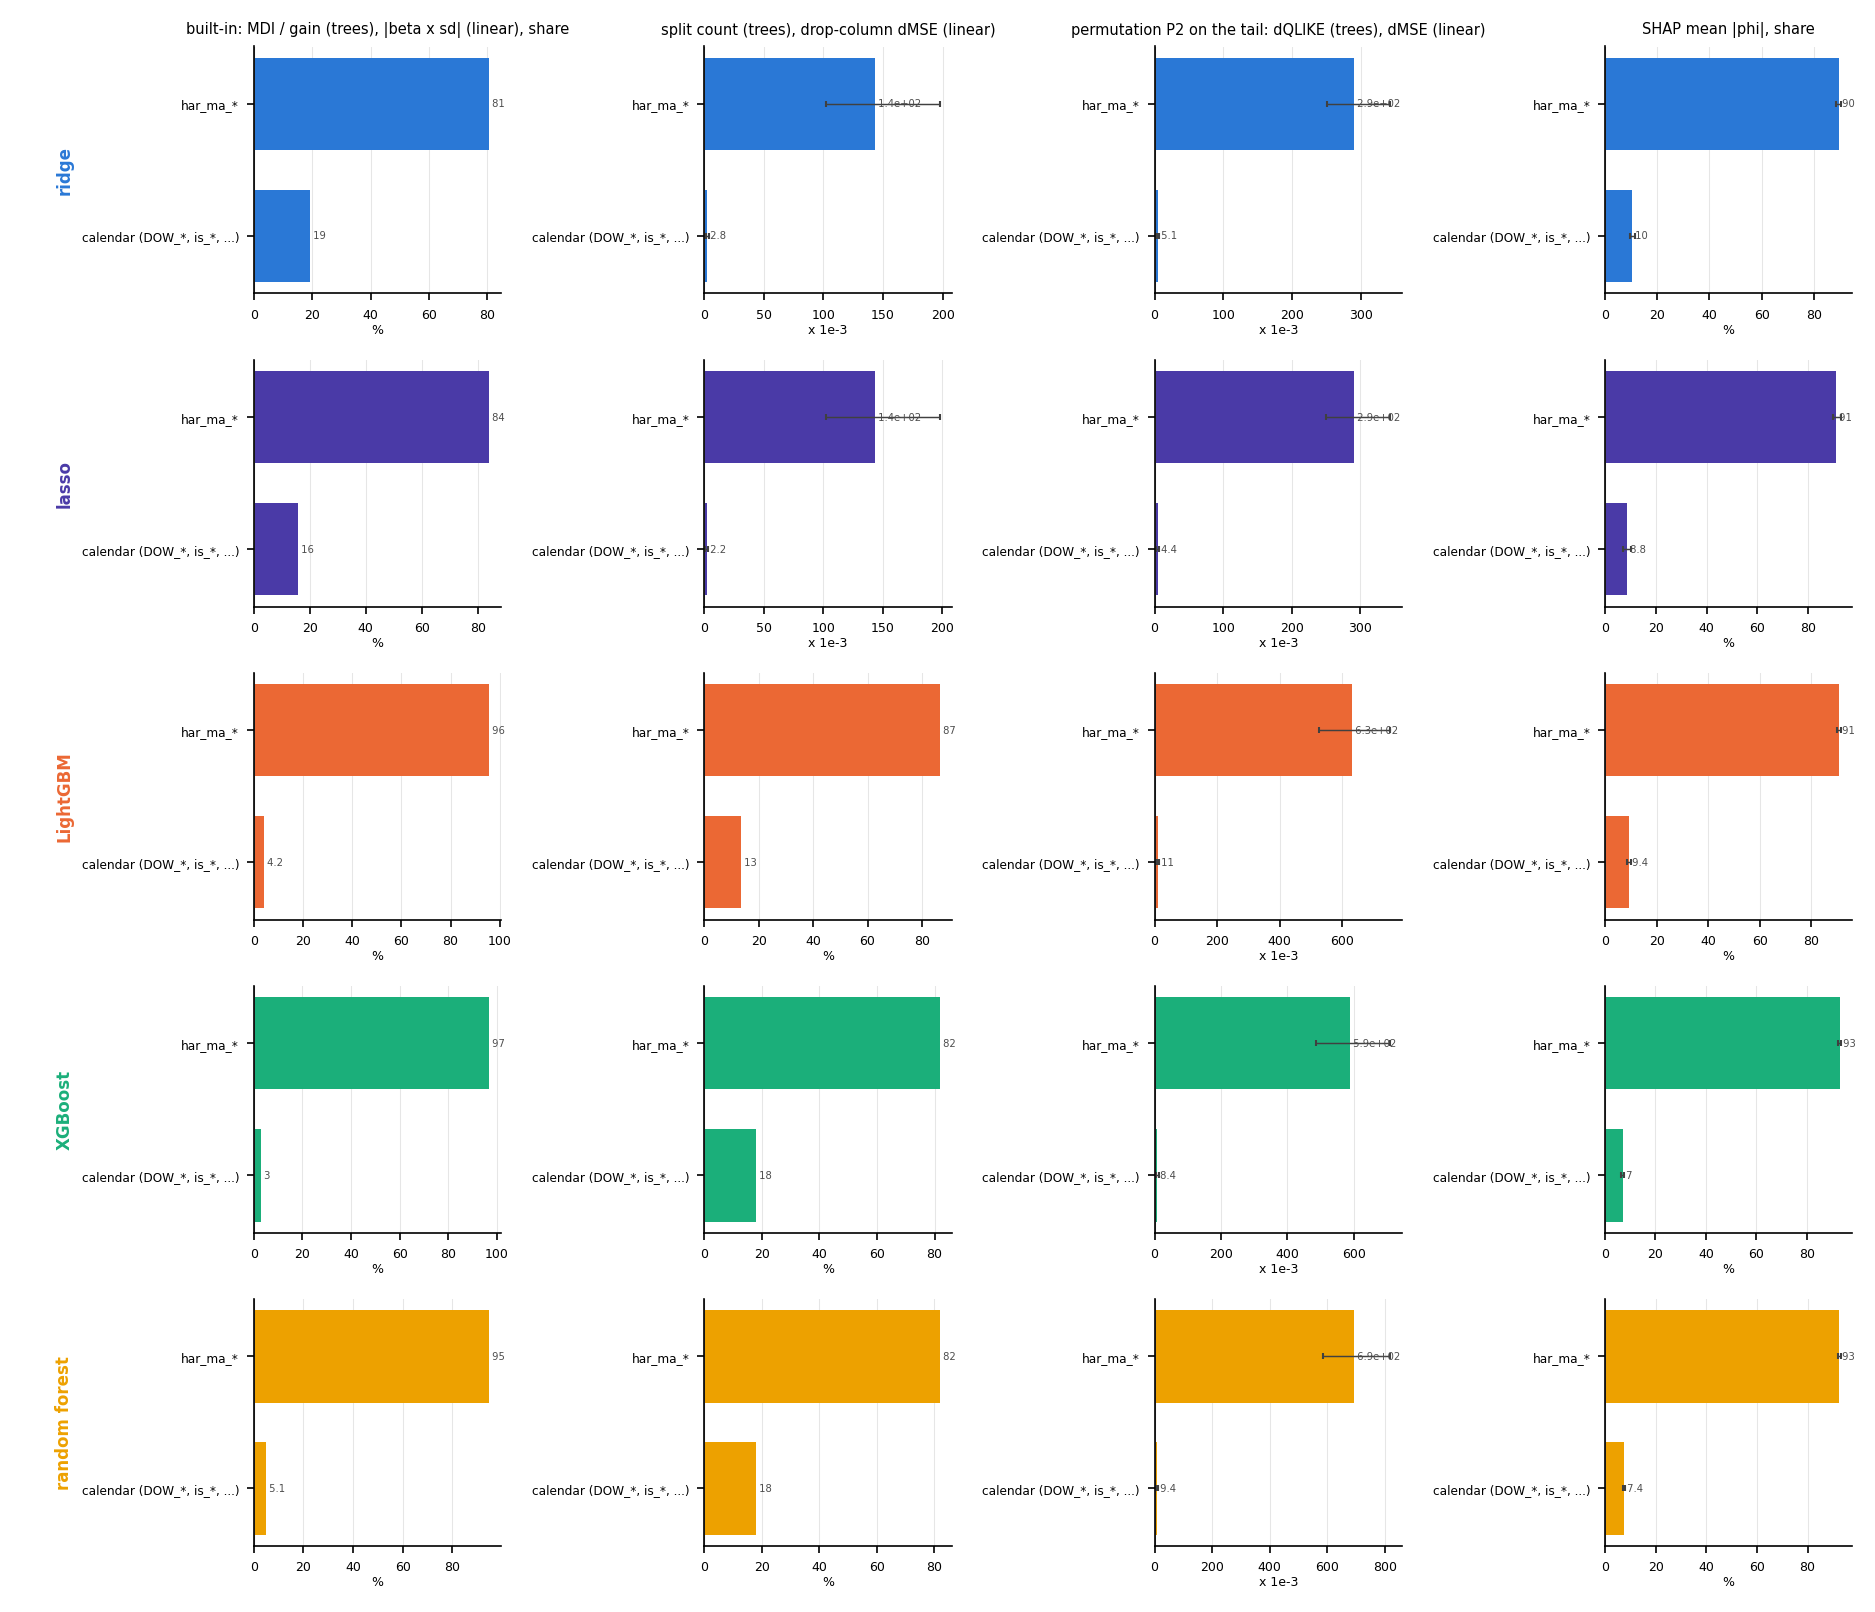
\includegraphics[width=\textwidth]{../results/feature_importance_1530/fig_ranked_baseline.png}
\caption{HAR + calendar: ranked bars per measure.}\end{figure}
\begin{figure}[H]\centering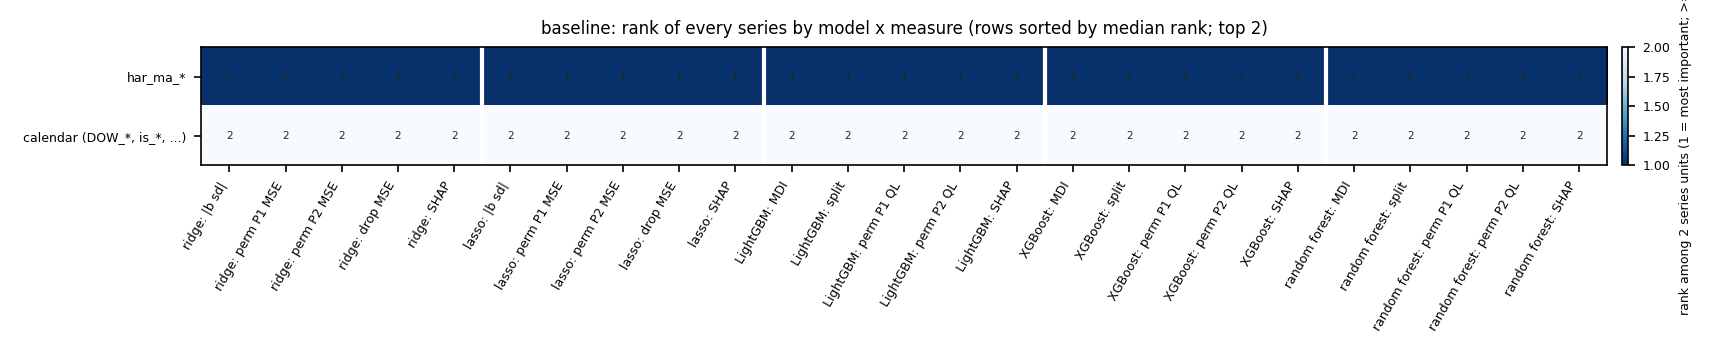
\includegraphics[width=0.7\textwidth]{../results/feature_importance_1530/fig_rank_heatmap_baseline_series.png}
\caption{HAR + calendar: ranks across measures.}\end{figure}
\begin{figure}[H]\centering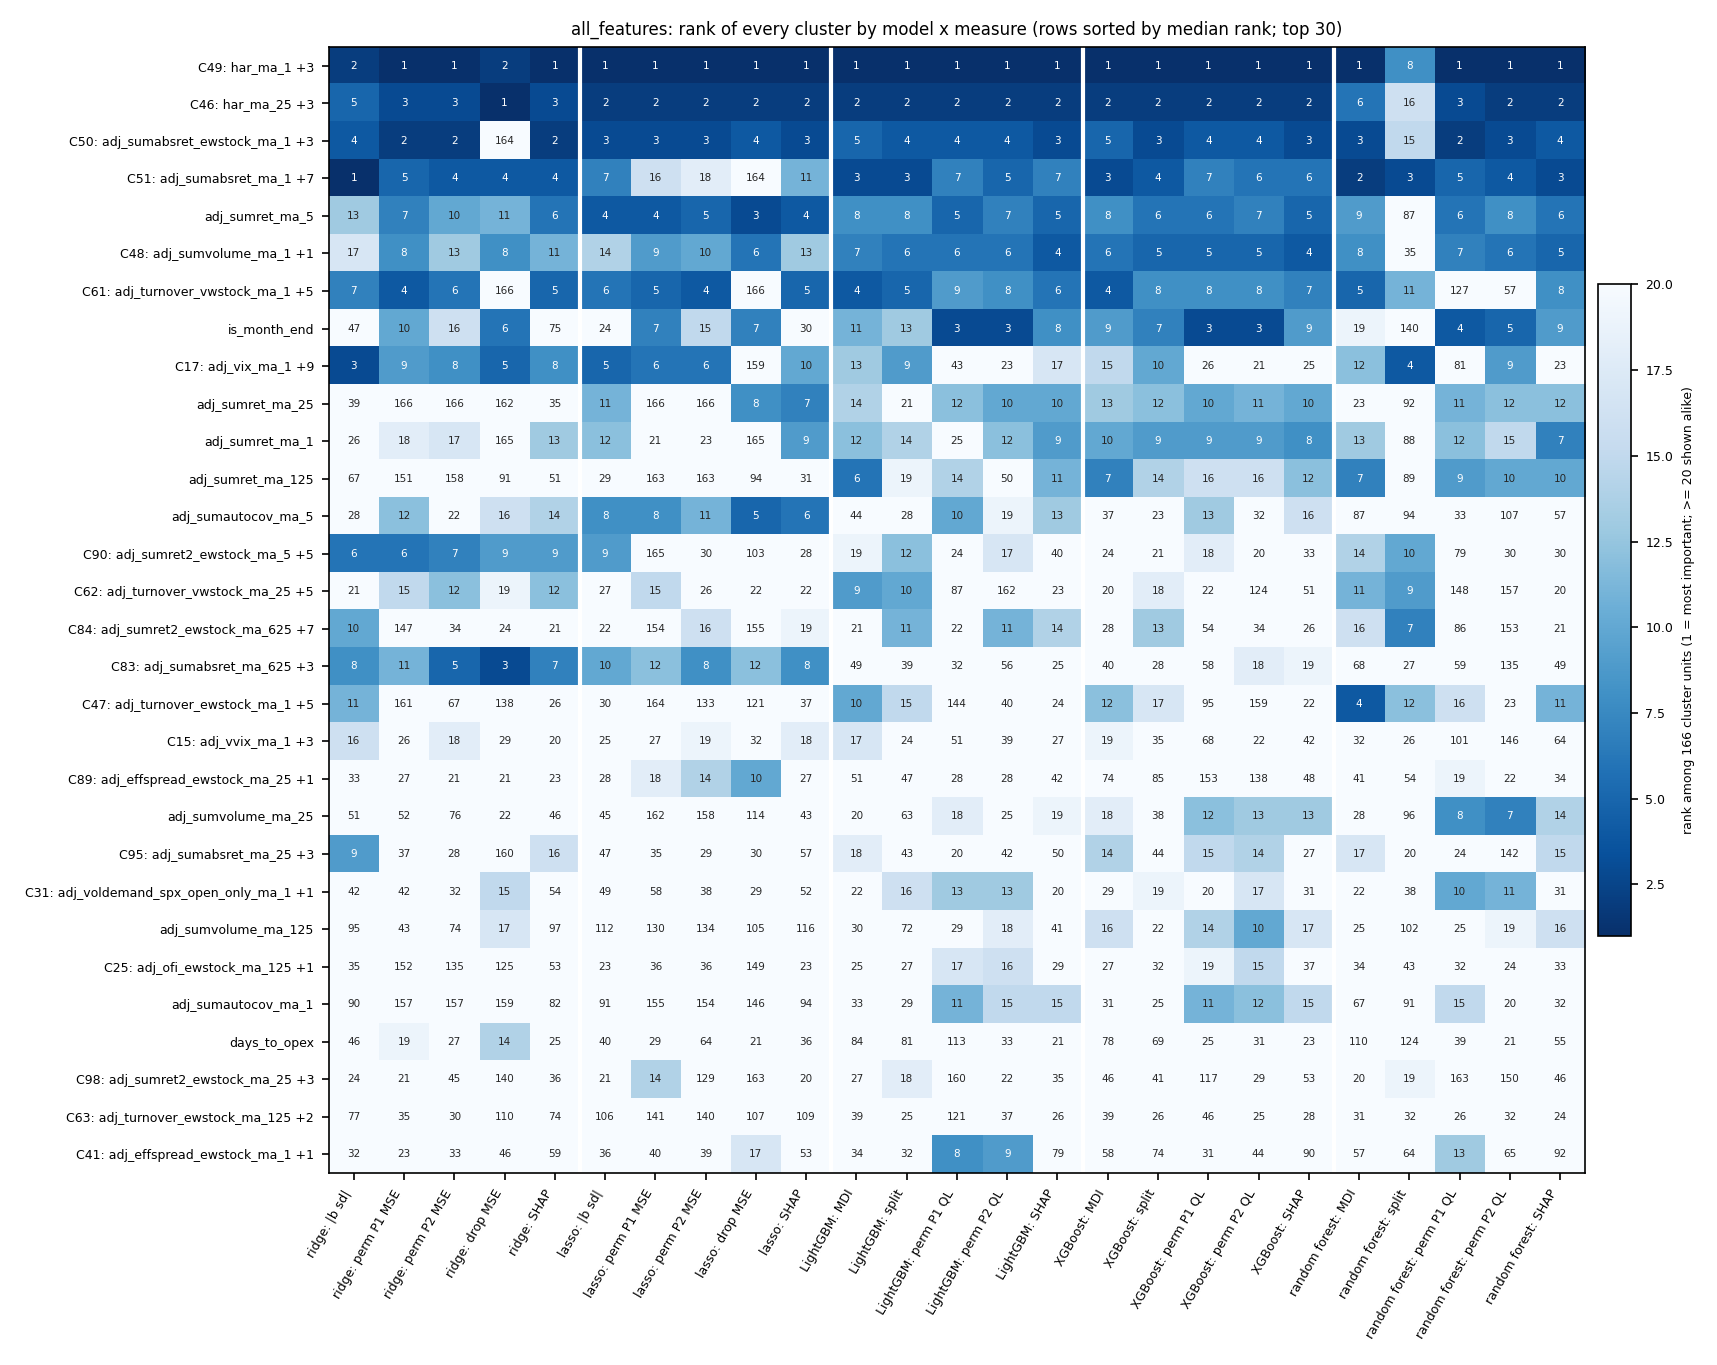
\includegraphics[width=0.95\textwidth]{../results/feature_importance_1530/fig_rank_heatmap_all_features_cluster.png}
\caption{All features: ranks at the cluster level.}\end{figure}

\end{document}
